\ifx\PREAMBLE\UnDef
\documentclass{beamer}
\usepackage{tikz}
\usepackage[english]{babel}
% or whatever

\usepackage[latin1]{inputenc}
% or whatever
\usepackage{xifthen}
\usepackage{bsymb}
\usepackage{eventB}

\newcommand{\always}{\mathop{\square}}
\newcommand{\eventually}{\mathop{\diamondsuit}}
\newcommand{\until}{\mathop{\mathcal{U}}}

\begin{document}
\else
\fi

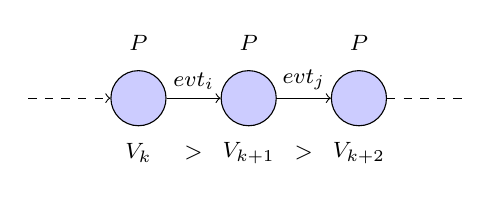
\begin{tikzpicture}[scale=0.7]
  \footnotesize
  \draw (0,0) node(s0)[circle, draw, inner sep =
  2pt, fill=blue!20!white, minimum width=0.7cm]{};
  \draw (2,0) node(s1)[circle, draw, inner sep =
  2pt, fill=blue!20!white, minimum width=0.7cm]{};
  \draw (4,0) node(s2)[circle, draw, inner sep =
  2pt, fill=blue!20!white, minimum width=0.7cm]{};
  \draw[->,dashed] (-2,0) -- (s0);
  \draw[->] (s0) --node[above]{$\Bevt{evt_i}$} (s1);
  \draw[->] (s1) --node[above]{$\Bevt{evt_j}$} (s2);
  \draw[dashed] (s2) -- (6,0);
  \draw (0,1) node{$\structure{P}$};
  \draw (2,1) node{$\structure{P}$};
  \draw (4,1) node{$\structure{P}$};

  \draw (0,-1) node{$\alert{V_{k}}$};
  \draw (1,-1) node{\alert{$>$}};
  \draw (2,-1) node{$\alert{V_{k+1}}$};
  \draw (3,-1) node{\alert{$>$}};
  \draw (4,-1) node{$\alert{V_{k+2}}$};
\end{tikzpicture}

\ifx\PREAMBLE\UnDef
\end{document}
\else
\fi
